\documentclass[b5paper,opensource,sourcefont,parskip]{qyxf-book}
\usepackage{subcaption}
\usepackage{draftwatermark}
\usepackage{fontawesome5}
\SetWatermarkText{钱院学辅}
\SetWatermarkLightness{0.92}
\SetWatermarkScale{0.9}

% --------------------警告--------------------
% 由于副标题较长,因此私自在使用的qyxf-book.cls
% 文件中将副标题的字体尺寸由 \Huge 改为了 \huge,
% 请其他人编译时注意。
% --------------------------------------------

\title{大学物理(上)题解·阶段二}
\subtitle{Key to University Physics Volume One: Part \uppercase\expandafter{\romannumeral2}}
\author{钱院学辅大物编写小组}
\typo{钱院学辅排版组}
\date{2019 年 6 月 9 日}
\version{v1.0}
\sourcepage{\url{https://github.com/qyxf/BookHub/}}

\graphicspath{{figs/}}

\newcommand{\di}[1]{\mathrm{d}#1}
\newcommand{\p}[2]{\frac{\partial #1}{\partial #2}}
\newcommand{\pp}[2]{\frac{\partial ^2 #1}{\partial #2 ^2}}
\newcommand{\dy}[2]{\frac{\di{#1}}{\di{#2}}}
\newcommand{\ddy}[2]{\frac{\mathrm{d} ^2 #1}{\mathrm{d} #2 ^2}}
\newcommand{\zbj}[4]
{
	\draw (0,0) node[below left] {$ O $};
	\draw [->] (#1,0) -- (#2,0) node[right] {$ x $};
	\draw [->] (0,#3) -- (0,#4) node[right] {$ y $};
}

\usepackage{siunitx}%输入角度
\usepackage{color}
\renewcommand{\thefootnote}{\color{red}\arabic{footnote}}%更改脚注格式

\begin{document}
\maketitle

\pagestyle{plain}
\chapter*{前言}
大学物理(University Physics)是本校理工科学生在大一、大二年级所要学习的一门自然科学
基础课程。这门课程课时较多、内容丰富,相关的练习题与考试题则尤显花样繁多,充分考验着每一个
学生对相关知识的掌握程度与应用能力。从掌握知识的角度来说,多做、精做大物习题是学好这门
课程的必经之路;从备考、应试的角度来说,若不熟练掌握各类大物习题的思路与解法,而仅依靠课内所
学到的基本知识点,则不可能在考试中取得令人满意的成绩。因此,熟练掌握本课程相关练习题的
解题技巧,是非常必要的。

目前,大多数大学物理的课堂均以一套统一印制的活页练习题作为课下作业。这套题目按章布置,
每章均有选择题、填空题、计算题三个部分,题量适中,覆盖了各章所有较为重要的知识点,并能
够使同学们充分地将课上所学知识用于实际问题的解决过程中。基于种种原因,这份题目的答案未见
公开;这能够保证大多数同学独立地完成作业,但不利于大家检查错误、在参考过程中发现自己的
问题。

为了解决这一问题,自2019年3月以来,钱院学辅组织了一些正在学习本课程的同学,编写了这份
大学物理题解(目前仅涵盖上半学期的相关内容)。该题解囊括了这一学期布置的所有作业之题解,
均有较详细的分析与求解过程可供参考。全书始终采用\LaTeX 整理,这使得本题解的排版效果得到
了充分的保证。我们希望,这份精心制作的题解,能够给正在学习与将要学习这门课程的同学提供
充分的帮助,使他们能够更好的掌握这项重要的基础课之内容。

本题解由\textbf{钱院学辅大物编写小组}完成,成员包括(按姓名拼音顺序):钱学森84班费立涵、
化生81班高旭帆、钱学森84班李浩天。其中,费立涵编写了第二、四、七章及第
一章计算题部分,李浩天编写了第三、五、八章,高旭帆编写了第六、九章及第一章的选择题与填空
题部分。钱院学辅学研部的越杰81班唐智亿、自动化钱71班吴思源与能动少C71班尤佳睿参加了稿件
的整理、校对、汇总与发布工作。在此,应向这些同学——特别是花费课余时间撰写题解的同学们表示
感谢。

“不积跬步,无以至千里。”一份可靠的题解,需要经过多次的改进才可望真正铸造出来。虽然这份题解的确可谓“精心制作”,但笔误、错漏等在所难免,特别需要各位使用者帮助我们指正。如您在参考的过程中发现有任何错误
之处,欢迎您通过下面的方式联系我们,帮助我们改进这份题解:
\begin{itemize}
	\item \faGithub ~~ GitHub平台论坛(\textbf{推荐,但需要注册}):\url{https://github.com/qyxf/BookHub/issues}
	\item \faInternetExplorer ~~ 钱院学辅信息发布站:\url{https://qyxf.github.io}
	\item \faEnvelopeOpen ~~ 钱院学辅邮箱:\texttt{qianxiaofu.mail@qq.com}
	\item \faQq ~~ 钱院学辅官方答疑墙:~~\textbf{钱小辅}~~206713407
\end{itemize}

作为钱院学辅出品的第一份“重量级”作品,希望它能够带给每一位同学最好的体验!

\begin{flushright}
钱院学辅大物编写小组\\
2019 年 6 月 9 日
\end{flushright}
\vspace{1.0cm}
\begin{figure}[!h]
	\centering
	\begin{minipage}[c]{0.5\textwidth}
		\centering
		
\includegraphics[scale=0.5]{qrcode2.png}
	\end{minipage}%
	\begin{minipage}[c]{0.5\textwidth}
		\centering
		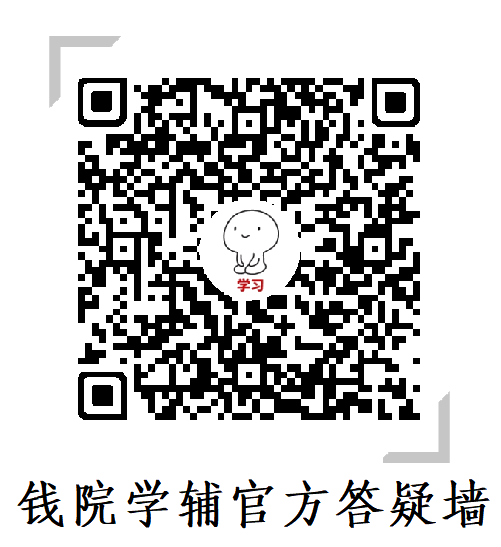
\includegraphics[scale=0.5]{qxf.png}
	\end{minipage}
\end{figure}


\cleardoublepage

\tableofcontents

\setlength{\parindent}{0pt}
\chapter{质点运动学及牛顿运动定律}
\section{选择题}
\exercise{1}A

\solve 如图1.1,对$M$,在$x$方向上:
\begin{figure}[htbp]
	\centering
	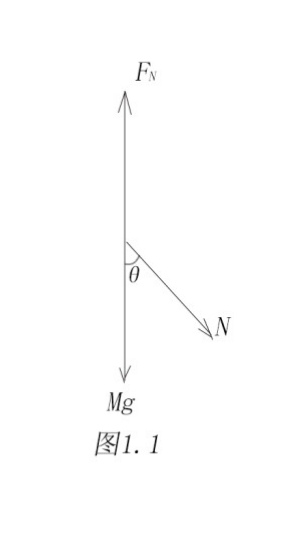
\includegraphics[width=10em,height=15em]{Chp1_illus1.png}
	\quad
	\centering
	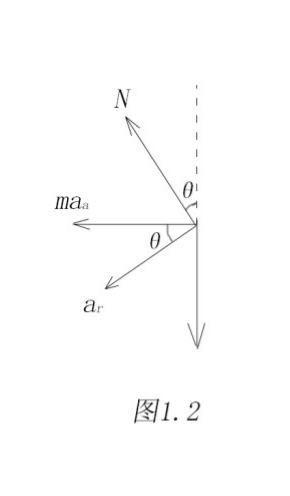
\includegraphics[width=10em,height=15em]{Chp1_illus2.png}
\end{figure}
\begin{equation}
N\sin\theta=Ma_e\text{(M对地)}
\end{equation}
如图1.2,对$m$,以$M$为参考系,$m$受一惯性力,合加速度沿二者接触面。沿$x,y$方向分解:
\begin{gather}
mg-N\cos\theta=ma_r\sin\theta\\
ma_e+N\sin\theta=ma_r\cos\theta
\end{gather}
将(1)代入(2),由(2)(3)联立解得:
\[a_r=\dfrac{(M+m)g\sin\theta}{M+m{\sin\theta}^2}\]


\exercise{2}B

\solve 如图1.3,$u=v\cos\theta$,v不变而$\theta$增大,需要u减小。

\begin{figure}[htbp]
	\centering
	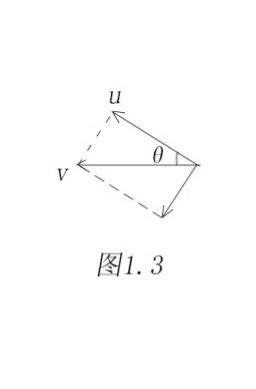
\includegraphics[width=6.5em,height=10em]{Chp1_illus3.png}
	%\caption{}
	\label{fig:Chp1_illus2}
\end{figure}


\exercise{3}A

\solve 匀速圆周运动的速度、加速度(受力)均是大小不变、方向时刻变化。
注意一个矢量为常量包括大小和方向两个方面。否则就是变化的量。

\exercise{4}B

\solve 以前面的货车为参考系,货车静止,火车速率为$v_1-v_2$,加速度为$a$(反向),那么火车最多前进$s=\dfrac{{(v_1-v_2)}^2}{2a}$。要求$d>s$,故选B。或采用地面参考系的追逐问题法,计算从$v_1\text{减速到}v_2$两车走过的距离之差为
\[
s=\dfrac{{v_1}^2-{v_2}^2}{2a}-v_2\cdot \dfrac{v_1-v_2}{a}=\dfrac{{(v_1-v_2)}^2}{2a}.
\]

\exercise{5}C

\solve 两次求导得:$a=30t$,不等于常数而大于零。

\exercise{6}B

\solve 求导得:$v=8t-6t^2,a=8-12t$

令$y=0\Rightarrow t=0\text{(舍去)或}2$s,代入得结果。

\exercise{7}B

\solve 物体做匀加速直线运动。
\begin{gather*}
s=\dfrac{b}{\cos\alpha},a=g\sin\alpha\\
t=\sqrt{\dfrac{2s}{a}}=\sqrt{\dfrac{4b}{g\sin(2\alpha)}}
\end{gather*}
当$t$最小时,$\sin(2\alpha)$最大,$\alpha=45^\circ$。

\exercise{8}B

\solve 类比从静止出发的匀加速直线运动。$\dfrac{1}{2}\beta t^2=2\pi$

\exercise{9}B

\solve 曲线的定义:“动点运动方向连续变化的轨迹\footnote{来源:汉典网http://www.zdic.net/c/2/111/299079.htm}”。A,C的反例:匀速圆周运动。做曲线运动的物体一定有加速度。

\exercise{10}D

\solve 反例:平抛运动。

\section{填空题}
\exercise{11}$0$\qquad$2g$

\solve 设A、B质量为m。抽走C之前,弹簧中的弹力大小为mg。撤去C时,弹簧长度未突变,弹力不变,A受合力为0;支持力则消失。

故$a_A=0$,$a_B=\dfrac{mg+mg}{m}=2g$,竖直向下。

\exercise{12}$\dfrac{25}{12}\pi$ rad/$\textrm{s}^2$ \qquad$\dfrac{24}{5} \textrm{s}$

\solve 简单公式应用。
\begin{gather*}
\text{}\theta=60\times2\pi=120\pi\\
\beta=\dfrac{\omega_2^2-\omega_1^2}{2\theta}=\dfrac{25}{12}\pi\ rad/s^2\\
\Delta t=\dfrac{\omega_2-\omega_1}{\beta}=\dfrac{24}{5}s
\end{gather*}

\exercise{13}$m(\sin\theta-\omega^2l\sin\theta\cos\theta)$

\begin{figure}[!htbp]
	\centering
	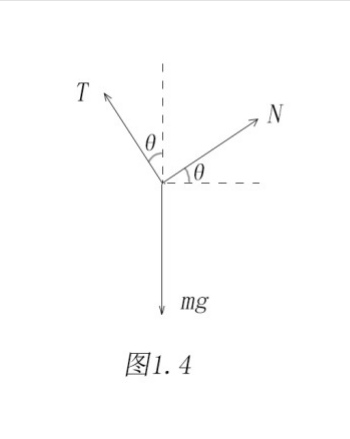
\includegraphics[width=15em, height=15em]{Chp1_illus4.png}
	%\caption{}
	\label{fig:c1}
\end{figure}

\solve 如图1.4,在$x$,$y$方向上分解受力,得:

\[\begin{cases}
T\sin\theta-N\cos\theta=m\omega^2l\sin\theta\\
T\cos\theta+N\sin\theta=mg
\end{cases}
\]
联立可解得$T$、$N$的大小。

\exercise{14}\ $2\sqrt{\dfrac{r}{g}}$ \qquad $2\sqrt{\dfrac{r}{g}}$

\solve 
设弦与PC的夹角为$\theta$,则有:
\begin{gather*}
s=2r\cos\theta,a=g\cos\theta\\
t=\sqrt{\dfrac{2s}{a}}=2\sqrt{\dfrac{r}{g}}
\end{gather*}
结果与$\theta$无关。


\exercise{15}$4\sqrt{5}\textrm{m/s}$ \qquad $16\textrm{m/s}^2$

\solve 抛物线的切线方向即为质点的速度方向,且$x=v_xt$。
\[
\dfrac{v_y}{v_x}=\dy{y}{x}=x\Rightarrow v_y=4x=16t
\]
$x=2$m时,$t=0.5$s,则:
\begin{gather*}
v_y=8\textrm{m/s}\\
v=\sqrt{{v_x}^2+{v_y}^2}=4\sqrt{5}\mathrm{m/s}
\end{gather*}
$v_x$不变,故:
\[
a=a_y=\dy{v_y}{t}=16\textrm{m/s}^2
\]

\exercise{16} 长度、质量、时间

\solve 见课本。

\exercise{17} 3\quad 3\quad 6

\solve $x$分别对$t$求一阶、两阶导,即是$v$、$a$,由图像即可判断其正负号。

\exercise{18} $y={(x+5)}^3$

\solve 由题,$x=2t-5\Rightarrow 2t=x+5$。

代入$y=8t^3={(2t)}^3$,消去t即可。

\exercise{19}$\dfrac{1}{2}g$\qquad 竖直向下

\solve 初始时受力平衡,两根弹簧上力均为$\dfrac{1}{2}mg$;一根断掉后,向上的力减半,则小球受的合力是$\dfrac{1}{2}mg$,竖直向下。

\exercise{20}$9$m/s

\solve 
\begin{align*}
\text{(SI)} x=3t+6t^2-2t^3&\xrightarrow{\text{求导}}v=3+12t-6t^2\\
&\xrightarrow{\text{求导}}a=12-12t
\end{align*}
令$a=0$,解得
\[
t=1\xrightarrow{\text{代入得}} v(1)=9\mathrm{m/s}
\]

\section{计算题}
\exercise{21}

\solve 
由图知:
\begin{gather*}
\tan\alpha=\dfrac{|\vec{a}_n|}{|\vec{a}_\tau|}=\dfrac{\frac{v^2}{R}}{\dy{v}{t}}\\
\frac{\di{v}}{v^2}=\frac{\di{t}}{R\tan\alpha}
\end{gather*}
积分得:
\[
-\frac{1}{v}=\frac{1}{R\tan\alpha}t+C
\]
代入$t=0,v=v_0$:
\[
C=-\dfrac{1}{v_0}\Rightarrow -\frac{1}{v}=\frac{t}{R\tan\alpha}-\dfrac{1}{v_0}
\]
所以:
\[
v=\frac{v_0R\tan\alpha}{R\tan\alpha-v_0t}
\]

\exercise{22}

\solve 
\begin{gather*}
\vec{v}=\dy{s}{t}\vec{\tau}=(c+2dt)\vec{\tau}\\  
\vec{a}_n=\frac{v^2}{R}\vec{n}=\frac{(c+2dt)^2}{R}\vec{n}\\
\vec{a}_\tau=\dy{v}{t}\vec{\tau}=2d\vec{\tau}
\end{gather*}
令$|\vec{a}_n|=|\vec{a}_\tau|$,则
\begin{gather*}
\frac{(c+2dt)^2}{R}=2d\\
t=t_1=\frac{\sqrt{2dR}-c}{2d}\left(t_2=\frac{-\sqrt{2dR}-c}{2d}<0\text{,舍去}\right)
\end{gather*}
$\therefore$要使$t\geqslant0$,条件为$\sqrt{2dR}-c\geqslant0$,即$2dR\geqslant c^2$。


\exercise{23}

\solve 根据已知条件有$-kx=a=\dy{v}{t}=\dy{v}{x}\cdot \dy{x}{t}=\dy{v}{x}\cdot v$,此即关于$x$与$v$的微分方程
\[-kx=\dy{v}{x}\cdot v\]
分离变量,积分得
\[-\dfrac{1}{2}kx^2=\dfrac{1}{2}v^2+C_1\]
令$C=2C_1$,则有$-kx^2=v^2+C$,进一步代入$x=x_0,v=v_0$得$C=-(kx_0^2+v_0^2)$。经过整理可得
\[v=\pm\sqrt{kx_0^2+v_0^2-kx^2}.\]


\exercise{24}

\solve (1) 易得$v=10\left(1-\dfrac{t}{5}\right)=-2t+10$,此即
\[
\dy{x}{t}=-2t+10
\]
积分得$x=-t^2+10t+c$,代入$t=0,x=0$可求得$c=0$。故有
\[x=-t^2+10t\]
代入$t=10s$得$x(10)=0$,即坐标为0。\\
(2) 令$x=10$m,则有$t^2-10t+10=0$,解得
\[t=5\pm\sqrt{15}\text{ s}\]
同理,令$x=-10$m,有$t^2-10t+10=0$,解得
\[t=5+\sqrt{35}(5-\sqrt{35}<0,\text{舍去})\]
综上可知,时刻为$5-\sqrt{15}$\ s,$5+\sqrt{15}$\ s或$5+\sqrt{35}$\ s。\\
(3) 令$v=0$,有$t=5$s,故可见对t\in[0,5],有$s=x=-t^2+10t$;而对$t\in[5,+\infty)$,有
\[s=s(5)+[s(5)-x]=25+[25-(-t^2+10t)]=t^2-10t+50\]
综上得$s=
\begin{cases}
-t^2+10t,&t\in[0,5)\\
t^2-10t+50,&t\in[5,+\infty)
\end{cases}$

\chapter{功和能}
\section{选择题}

\exercise{1}C

\solve 质点沿力方向位移为零,故$A=0$.

\exercise{2}B

\solve 可见$B$离开$A$时为弹簧恢复原长的时刻(该时刻之后,$A$受到弹簧拉力,加速度为负,$v_A<v_B$.),
此时$v_A=v_B$.由动能定理易得
\[\frac{1}{2}mv_A^2+\frac{1}{2}mv_B^2-0=\frac{1}{2}kd^2\]
故$E_B=\frac{1}{2}mv_B^2=\frac{1}{4}kd^2$.


\exercise{3}C

\solve 对$\vec{r}$求导得$\vec{v}=\frac{\di{\vec{r}}}{\di{t}}=-\frac{2\pi}{T}A\sin\frac{2\pi t}{T}\vec{i}+\frac{2\pi}{T}B\cos\frac{2\pi t}{T}\vec{j}$.
$t=0$时,有
\[
v_1=\sqrt{v_{x1}^2+v_{y1}^2}=\sqrt{0^2+\left(\frac{2\pi}{T}B\right)^2}=\frac{2\pi}{T}B
\]
故$E_{k1}=\frac{1}{2}mv_1^2=\frac{2m\pi^2}{T^2}\left(B^2\right)$.而$t=\frac{T}{4}$时,
\begin{align*}
v_2&=\sqrt{v_{x2}^2+v_{y2}^2}\\
&=\sqrt{\left(-\frac{2\pi}{T}A\right)^2+0^2}=\frac{2\pi}{T}A
\end{align*}
故$E_{k2}=\frac{1}{2}mv_2^2=\frac{2m\pi^2}{T^2}\left(A^2\right)$,从而
\[\Delta{}E_k=\frac{2\pi^2}{T^2}(B^2-A^2)\]


\exercise{4}D

\solve 由动量定理:
\[0=m_1v_1-m_2v_2\]
\[\therefore{}v_2=\frac{m_1}{m_2}v_1\]

由机械能守恒:
\begin{align*}
E_p &=\frac{1}{2}m_1v_1^2+\frac{1}{2}m_2v_2^2\\
&=\frac{m_1v_1^2+\frac{m_1^2v_1^2}{m_2}}{2}\\
&=\frac{m_1v_1^2\left(m_1+m_2\right)}{2m_2}
\end{align*}

\exercise{5}B

\solve (2):既然小车能在水平面上停止,说明水平面是粗糙的,有摩擦力做功。因此不满足机械能守恒。

(4):重力做正功,摩擦力做负功,符号相反。

\exercise{6}D

\solve 弹簧上任意一点弹力相同,记为N。截去一半后,伸长量缩短了一半,而弹力不变,因此k变为原来的两倍。并联在一起后,每一根弹簧受力为原先的一半。由$F=kA$,伸长量为原来的$\frac{1}{4}$。写成数学式子如下:
\[
E_k=2\times\left(\frac{1}{2}k'A'^2\right)=\left(2k\right)\times\left(\frac{1}{4}A\right)^2=\frac{1}{8}kA^2
\]

\exercise{7}D

\solve 物体沿重力方向的位移为负,因此重力做负功。其它选项,物体沿推力方向有位移,因此推力做功,A错误;推力功与摩擦力做的功和重力做的功之和等值反号,因此BC错误。

\exercise{8}C

\solve 若合外力的冲量为0,则由冲量定义$\vec{I}=\int_{t_1}^{t_2}\vec{F}\di{t}$知,$\vec{F}=\vec{0}$,因此合外力做的功为0。其它选项,AD可举匀速圆周运动的反例;对于B,合外力不为0,必有加速度,而质量不改变,因此$\vec{v}$必然改变,即动量必改变。\\

\exercise{9}B

\solve 由动能表达式$E_k=\frac{p^2}{2m}$,在动量相同的情况下,质量越大,动能越小,因此选B\\

\exercise{10}A

\solve 设小球重力为$G$,弹簧弹性系数为$k$,则$G=kd$,再设最低点时弹簧伸长$h$。以弹簧原长的高度为基准,释放前和最低点为始末态,应用机械能守恒:
\[Gh=\frac{1}{2}kh^2\]
解得$h=2d.$

\section{填空题}

\exercise{11}$31J$

\solve $A=\int_{0.5}^{1}F\di{x}=\int_{0.5}^{1}(52.8x+38.4x^2)\di{x}=31(J)$

\exercise{12}$24J$ $4m/s$

\solve $A=\int_{1}^{4}F\di{x}=\int_{1}^{4}(3+2x)\di{x}=24(J)$
由动能定理得$\frac{1}{2}mv^2=24,\quad \therefore v=4(m/s)$.

\exercise{13}$\frac{GMm}{6R}$ \qquad $-\frac{GMm}{3R}$

\solve 卫星运动的向心力由万有引力提供,故有
\[m\frac{v^2}{3R}=G\frac{Mm}{(3R)^2}\]
故有
\begin{gather*}
E_k=\frac{1}{2}mv^2=\frac{GMm}{6R}\\
E_p=-\frac{GMm}{r}=-\frac{GMm}{3R}
\end{gather*}

\exercise{14}1296

\solve
由牛顿第二定律$F=ma$,代入相关表达式有
\[t^2=2a=2\ddy{x}{t}\]
再由初始条件$t=0,x=0$且$v=0$,解得
\[x=\frac{1}{24}t^4\]
由此可知,$x=54$m时$t=6s$,故可以积分得到
\[A=\int_{0}^{6}F\di{x}=\int_{0}^{6}t^2\di{(\frac{1}{24}t^4)}=1296\text{(J)}\]


\exercise{15}$19.8m/s$

\solve
(小行星的物理量下标为1)向心力由万有引力提供,故$m\frac{v_1^2}{R_1}=G\frac{Mm}{R_1^2}$。将$M=\frac{4}{3}\pi R^3\rho$代入,得
\[v_1=\sqrt{G\frac{4}{3}\pi\rho R_1^2}\]
在地球上$g=9.8$m/s,故由重力的两种计算方法可以得到
\[mg=G\frac{Mm}{R_2^2}\]
从而$g=G\frac{4}{3}\pi R_2\rho$,进一步有$G\frac{4}{3}\pi\rho=\frac{g}{R_2}$
代入(1)即得$v_1=\sqrt{\frac{gR_1^2}{R_2}}\approx19.8$(m/s).

\exercise{16} $\sqrt{\frac{2Mgh}{m+M}}$ \qquad $\frac{m^2gh}{M+m}$

\solve 由动量定理,有
\begin{equation}
mv_1=Mv_2
\end{equation}
由机械能守恒,有
\begin{equation}
mgh=\frac{1}{2}mv_1^2+\frac{1}{2}Mv_2^2
\end{equation}
联立(1)(2)解得:$v_1=\sqrt{\frac{2Mgh}{m+M}}
,v_2=\sqrt{\frac{2m^2gh}{(m+M)M}}$。由动能定理知,物块对滑道做的功就是滑道动能改变量
\[\Delta E_k=\frac{1}{2}Mv_2^2=\frac{m^2gh}{M+m}\]

\exercise{17} 第$i$个质点所受合力做的功(类似说法均正确)

\exercise{18}1m/s \qquad 200J

\solve 船员用$200$N的力拉绳子,由牛顿第三定律,绳子也给船员(和船)$200$N的拉力。以人和船为对象应用牛顿第二定律,解得:
\[a=\frac{F}{m}=0.5\text{m/s}^2\]
因此第2秒末速率为1m/s,增加的动能就是
\[E_k=\frac{1}{2}mv^2=\frac{1}{2}\times400\times1^2=200(J)\]

\exercise{19}$\left(\frac{1}{r_2}-\frac{1}{r_1}\right)GMm$ 

\solve 由机械能守恒,$0+E_{p1}=E_k+E_{p2}$,故
\[E_k=E_{p2}-E_{p1}=\left(\frac{1}{r_2}-\frac{1}{r_1}\right)\]
以两个质点为系统,仅有万有引力(内力)做功,因此由质点系动能定理可得
\[A=E_k=\left(\frac{1}{r_2}-\frac{1}{r_1}\right)GMm\]

\exercise{20}$0.8\sqrt{2}$

\solve 参照下面的图\ref{fig:t20},功可直接按定义计算为:

\begin{figure}[htbp]
	\centering
	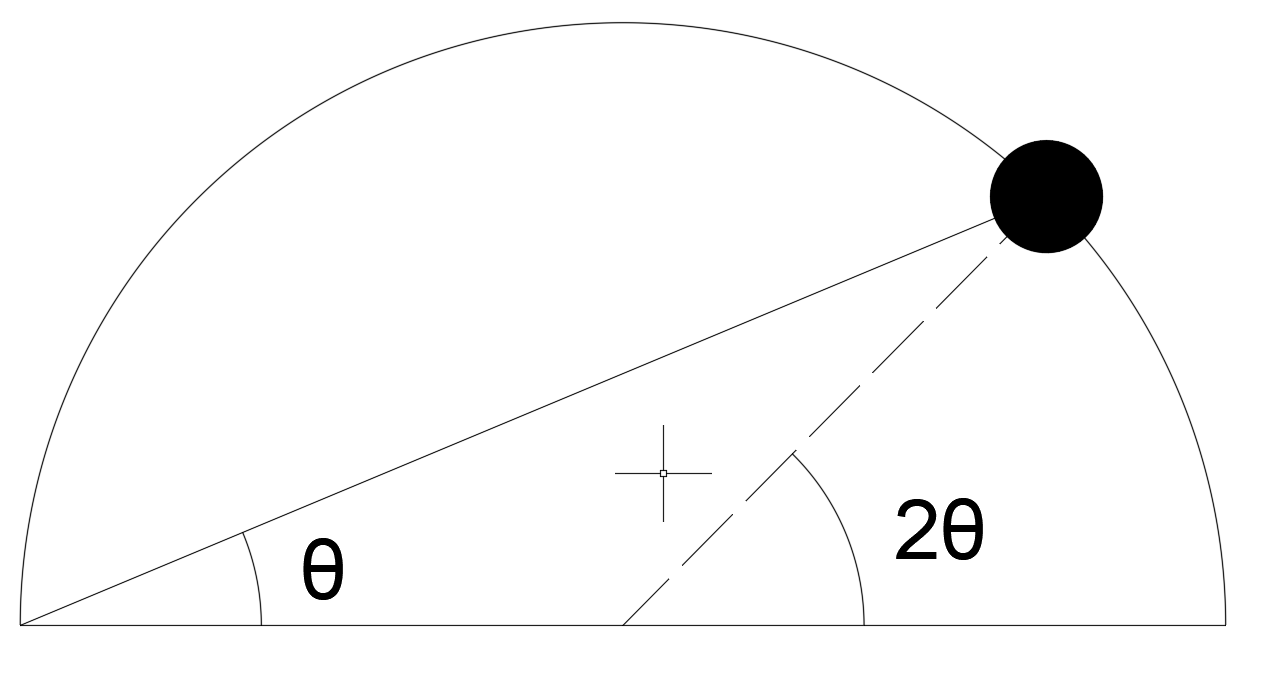
\includegraphics[height=100pt]{Chp2_illus1.png}
	\caption{练习20示意图}\label{fig:t20}
\end{figure}

\begin{align*}
A&=\int_{\theta=0}^{\theta=\frac{\pi}{4}}{\vec{F}}\cdot\di{\vec{x}}\\
&=\int_{\theta=0}^{\theta=\frac{\pi}{4}}F\di{x}\cos\left(\frac{\pi}{2}-\theta\right)\\
&=\int_{0}^{\frac{\pi}{4}}k(2R\cos\theta-0.1)\times\di{(R\times 2\theta)}\times\sin\theta\\
&=\int_{0}^{\frac{\pi}{4}}(-4R^2k\cos\theta+0.2Rk)\di{(\cos\theta)}\\
&=-2R^2k\cos^2\theta+0.2Rk\cos\theta\left.\right|_0^{\frac{\pi}{4}}\\
&=-2\times 0.2^2\times 40\times({\frac{\sqrt{2}}{2}}^2-1^2)+0.2\times 0.2\times 40\times(\frac{1}{2}-1)\\
&=0.8\sqrt{2}
\end{align*}


\section{计算题}
\exercise{21}

\solve 分别求解。

(1) 首先,有$\Delta l=\frac{F}{k}$,进而可得$E_p=\frac{1}{2}k(\Delta l)^2=\frac{F^2}{2k}$.由机械能守恒,可列出
$E_k-0=E_p-0$,代入各条件得
\[\frac{1}{2}Mv_{\text{右}}^2=\frac{F^2}{2k}\]
故得$v_{\text{右}}=\frac{F}{\sqrt{Mk}}$.

(2) 由受力分析知,$a_{\text{左}}=a_{\text{右}}$,即
\[\dy{v_{\text{左}}}{t}=-\dy{v_{\text{右}}}{t}\]
两边积分便得$v_{\text{左}}=-v_{\text{右}}+c$,代入刚恢复原长时的条件$v_{\text{左}}=0,v_{\text{右}}=\frac{F}{\sqrt{Mk}}$得
\[v_{\text{左}}+v_{\text{右}}=\frac{F}{\sqrt{Mk}}\]
故可见当$v_{\text{左}}=v_{\text{右}}$时,$v'_{\text{左}}=v'_{\text{右}}=\frac{F}{\sqrt{2Mk}}$。由机械能守恒可进一步得到
\[0+\frac{1}{2}M(v_{\text{右}})^2=\frac{1}{2}k(\Delta l)^2+\frac{1}{2}M(v'_{\text{左}})^2+\frac{1}{2}M(v'_{\text{右}})^2\]
解得$\Delta l=\pm\sqrt{\frac{M\left(\frac{F^2}{Mk}-2\times\frac{F^2}{4Mk}\right)}{k}}=\pm\frac{\sqrt{2}}{2}\frac{F}{k}$,即伸长或压缩$\frac{\sqrt{2}}{2}\frac{F}{k}$。

\exercise{22} 

\solve 记$x$为链条右端的位移,$l$为桌边链条的长度。据功的定义,有$\di{A}=F\cdot\di{x}=F\di{x}$;而当链条被匀速拉起,可知
\[F=G=M'g=\frac{l}{L}Mg\]
由几何意义,$\di{x}=-\di{l}$,故得
\[
A=\int_{\frac{L}{3}}^{0} -\frac{l}{L}Mg\di{l}
=\frac{Mg}{2L}l^2\left.\right|_{0}^{\frac{L}{3}}
=\frac{MgL}{18}
\]
如果有摩擦力$f$,则只需计算新的力
\[
F'=G+f=\frac{l}{L}Mg+\mu\left(\frac{L-l}{L}Mg\right)=\frac{Mg}{L}[\mu L+(1-\mu)l]
\]
进而就有
\begin{align*}
A&=\int_{\frac{L}{3}}^{0} -\frac{Mg}{L}[\mu L+(1-\mu)l] \di{l}=\frac{Mg}{L}\left.\left(\mu Ll+\frac{1-\mu}{2}l^2\right)\right|_{0}^{L/3}\\
&=\frac{Mg}{L}\left(\frac{\mu}{3}L^2+\frac{1-\mu}{18}L^2\right)=MgL\frac{5\mu +1}{18}
\end{align*}

\exercise{23}

\solve 首先,由图\ref{fig:t23-1},对小球应用牛顿第二定律:
\[m\dfrac{v^2}{R}=mg\cos\theta-N\]

\begin{figure}[htbp]
	\centering
	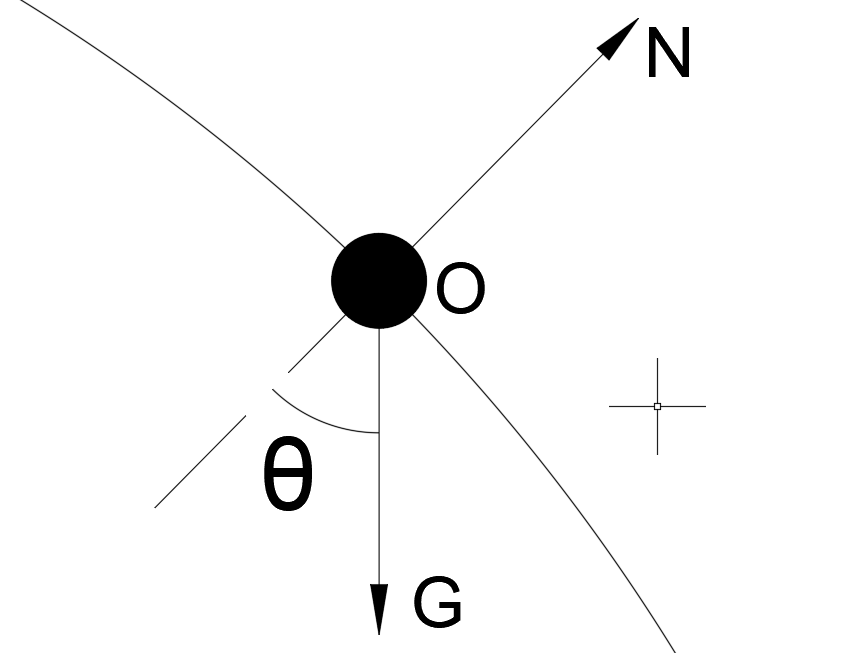
\includegraphics[height=100pt]{Chp2_illus2.png}
	\caption{练习23示意图1}\label{fig:t23-1}
\end{figure}

由受力分析(参见图\ref{fig:t23-2})知,圆环竖直方向受力$F$为
\[
F=(N'+N')\cos\theta=2N\cos\theta
\]

\begin{figure}[htbp]
	\centering
	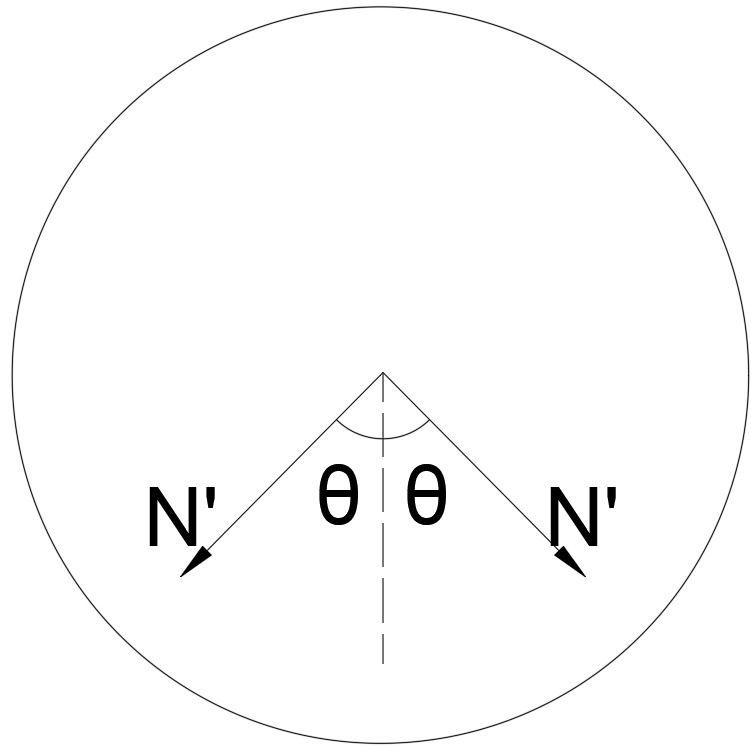
\includegraphics[height=100pt]{Chp2_illus3.png}
	\caption{练习23示意图2}\label{fig:t23-2}
\end{figure}

当$\theta\in[0,\frac{\pi}{2}]$时,$\cos\theta>0$,故当$N<0$时,$F$向上,圆环上升。从而有
\[N=mg\cos\theta-m\frac{v^2}{R}<0\]
由机械能守恒(见图\ref{fig:t23-3})得
\[\frac{1}{2}mv^2=mgh=mg(1-\cos\theta)R\]

\begin{figure}[htbp]
	\centering
	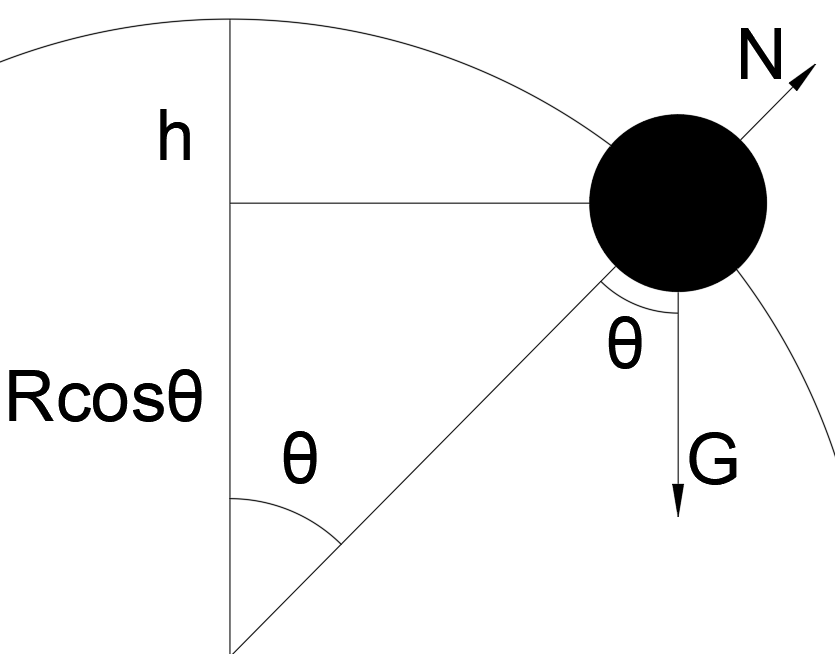
\includegraphics[height=100pt]{Chp2_illus4.png}
	\caption{练习23示意图3}\label{fig:t23-3}
\end{figure}

代入$N<0$的条件便得
\[mg\cos\theta-2mg(1-\cos\theta)<0\]
化简得$3\cos\theta<2$,解得$\theta>\arccos\frac{2}{3}$。即当$\theta>\arccos\frac{2}{3}$时,圆环会上升。

\exercise{24}

\solve $T_1$提供$G1+G2$,故有$k_1\Delta l=(m_1+m_2)g$,解得
\[\Delta l=\frac{(m_1+m_2)g}{k_1}\]
由机械能守恒有:
\[-mgx+\frac{1}{2}k_1(\Delta l+x)^2+\frac{1}{2}m_1v^2=0+\frac{1}{2}k_1(\Delta l)^2+0\]
解得
$v=\sqrt{\frac{-kx^2-2(k_1\Delta l-m_1g)x}{m_1}}=\sqrt{-\frac{k_1}{m_1}x^2-\frac{2m_2g}{m_1}x}$.利用二次函数最大值为$\frac{4ac-b^2}{4a}$的性质即得其最大值
\[
v_{\text{max}}=\sqrt{\frac{0-\frac{4m_2^2g^2}{m_1^2}}{4\left(-\frac{k_1}{m_1}\right)}}=\sqrt{\frac{m_2^2g^2}{m_1k_1}}=\frac{0.3\times 9.8}{\sqrt{0.5\times 8.9\times 10^4}}=0.0139(m/s)
\]



\chapter{功、能、冲量与动量}
\section{选择题}

\exercise{1}A

\solve 小球受到重力和弹簧弹力做的功,动能不守恒。小球受到的合外力不为0,因此动量不守恒。

\exercise{2}D

\solve 两船在过程中受到了人的摩擦力的作用,合外力不为零,动量不守恒。

\exercise{3}C

\solve 碰撞前后两球动量守恒,因此总动量为0,说明碰撞前两球动量大小相同,方向相反。

\exercise{4}D

\solve 两球碰撞后一起运动,说明为完全非弹性碰撞,存在机械能损失,因此机械能不守恒。两球还受到了弹簧弹力作用,合外力不为零,动量不守恒。

\exercise{5}D

\solve 运动半周前后小球的速度大小不变,方向相反,因此冲量大小\(I=m\Delta v=2mv=2mr \omega\)。

\exercise{6}C

\solve A人向右跳落入B船后,由动量守恒,A船具有向左的速度,A人具有向右的速度,落入B船后使得A人,B人,B船都具有了向右的速度。B人再跳回A船后,由动量守恒,B人获得的动量朝左,A人和B船获得的动量向右,因此最终B船的速度向右,\(v_B>0\)。B人和A船的动量都向左,因此最终B人落入A船后,A船速度向左,\(v_A<0\)。

\exercise{7}A

\solve 由公式\(E=\frac{p^2}{2m}\),\(p_1=\sqrt{2mE}\),\(p_2=\sqrt{2\times 4m\times E}=2\sqrt{2mE}\)(此处\(p_1\),\(p_2\)均为大小)。由于两个质点面对面运动,\(p_1\)和\(p_2\)符号相反,因此系统动量大小为\(p=p_2-p_1=\sqrt{2mE}\)。

\exercise{8}A

\solve 小球转一周后速度大小和方向都与转前相同,因此动量增量为0,A对。由冲量定义式\(I=F\Delta t\),\(F\)和\(\Delta t\)均不为0,因此\(I\)也不为0,B错,同理可知C错误。在转动过程中小球速度的方向发生了改变,因此过程中动量不守恒,D错。

\exercise{9}C

\solve 小球下落直到与板碰撞之前,对小球分析,有\(v=\sqrt{2gh}\),对板和弹簧分析,设此时弹簧的压缩量为\(x_0\),由胡克定律有\(x_0=Mg/k\);此后对球与板的碰撞过程,有动量守恒\(mv=(m+M)v_0\),解得\(v_0=\frac{m}{m+M}\sqrt{2gh}\);此后,小球与板一起运动,设两者一起运动的距离为\(x\),由能量守恒可列出
\[\frac{1}{2}(m+M)v_0^2+(M+m)gx+\frac{1}{2}kx_0^2=\frac{1}{2}k(x+x_0)^2\]
代入数据解得\(x=\frac{mg}{k}(1+\sqrt{1+\frac{2kh}{(M+m)g}})\),所以选择C项。

\exercise{10}A

\solve 两球碰撞后以相同速度运动,则为完全非弹性碰撞,必有机械能损失,与完全弹性碰撞矛盾,A错误;若两球碰撞前速度大小相同,方向相反,则碰撞后速度互换,B正确;完全弹性碰撞的定义即为机械能守恒的碰撞,C正确;碰撞过程中动量守恒,D正确。

\section{填空题}
\exercise{11}$10m/s$

\solve 以人和船为系统,过程中所受外力为$ 0 $,因此动量守恒。有
\begin{equation*}
(m+M)v=m(v'+\frac{v}{2})+M\frac{v}{2} 
\end{equation*}
代入数据解得$ v'=10m/s $.

\exercise{12}$ m\sqrt{2gh} $ \hspace{2em} 竖直向下

\solve $(1)$由$ I=\Delta p=F\Delta t $,小球下落时间为$\Delta t=\sqrt{\frac{2h}{g}}$,下落过程所受合外力为$F=mg$,故动量增量为
\begin{equation*}
\Delta p=mg\cdot\sqrt{2h/g}=m\sqrt{2gh}
\end{equation*}

$(2)$由合外力(重力)方向竖直向下,可得动量增量方向竖直向下。

\exercise{13}$\frac{5}{3}N\cdot s$,方向与力的方向同向 \hspace{2em} $\frac{5}{6}$N

\solve 由冲量定义,$I = \int F \di t$,对于本题来说,$F$是时间的函数,所以有
\begin{equation*}
I = \int_0^1 2t \di t + \int_1^2 2(2-t)^2 \di t = \frac{5}{3}\text{N} \cdot \text{s}
\end{equation*}
平均冲力为
\begin{equation*}
\overline{F} = \frac{I}{t} = \frac{5}{6} \text{N}.
\end{equation*}

\exercise{14}$-m\vec{v}$

\solve 对全过程,由动量定理,$\vec{I} = \Delta \vec{p} = -m\vec{v}$。

\exercise{15}$2350$kg$\cdot$ m/s \hspace{2em} 与炮弹飞行方向相反

\solve 由动量定理,$I = \Delta p = m(v-v_0)$,代入数据得$I=2350$kg$\cdot$ m/s,因为炮弹为减速运动,所以冲量方向与炮弹飞行方向相反。

\exercise{16}$\frac{m+M}{m}\sqrt{2 \mu gs}$

\solve 设子弹刚发射时的速度为$v_0$,子弹射入木块后共速速度为$v$。对子弹射入木块的过程,有动量守恒$mv_0=(M+m)v$,此后木块和子弹共同运动,由动能定理可列出
\begin{equation*}
\frac{1}{2}(m+M)v^2=\mu (m+M)gs
\end{equation*}
代入数据解得
\begin{equation*}
v_0=\frac{m+M}{m}\sqrt{2 \mu gs}.
\end{equation*}

\exercise{17}$\sqrt{\frac{kMl_0^2}{(M+m)^2}}$ \hspace{2em} $\sqrt{\frac{M}{M+nm}}l_0$

\analysis 每次油滴落入容器等价于油滴与容器发生了一次完全非弹性碰撞,该过程满足动量守恒;此后直到下一滴油滴落入容器之前,整体运动满足能量守恒。

\solve 当弹簧第一次达到原长即容器第一次到达滴管下方(第一滴油滴未滴入)时,设容器速度为$v_0$,由能量守恒
\begin{equation*}
\frac{1}{2}Mv_0^2=\frac{1}{2}kl_0^2
\end{equation*}
可得
\begin{equation*}
v_0=\sqrt{\frac{k}{M}}l_0
\end{equation*}
再设第$n$滴油滴滴入容器后容器与油滴整体的速度为$v_n$;由动量守恒$P_0=P_n$,其中初状态动量$P_0=Mv_0$,第$n$滴油滴滴入后动量$P_n=(M+nm)v_n$,解得
\begin{equation*}
v_n=\frac{M}{M+nm}v_0
\end{equation*}
此后容器达到偏离$O$点的最大运动距离$x_n$过程中,由能量守恒,有
\begin{equation*}
\frac{1}{2}(M+nm)v_n^2=\frac{1}{2}kx_n^2
\end{equation*}
成立,从中可解出
\begin{equation*}
x_n=\sqrt{\frac{M+nm}{k}}v_n
\end{equation*}

故当$n=1$时,
\begin{equation*}
v_1=\sqrt{\frac{kMl_0^2}{(M+m)^2}}
\end{equation*}
滴入$n$滴油滴后,容器偏离$O$点的最大距离为
\begin{equation*}
x_n=\sqrt{\frac{M}{M+nm}}l_0.
\end{equation*}

\exercise{18}$m(\alpha\sin(\omega t)\vec{i}-(\beta\cos(\omega t)-\beta)\vec{j})$

\solve 由已知条件$a_x=\omega\alpha\cos(\omega t),a_y=\omega\beta\sin(\omega t)$,所以$v_x=\int a_x\di t=\alpha\sin(\omega t)+C_1$,$v_y=\int a_y\di t=-\beta\cos(\omega t)+C_2$,又由初始条件$t=0$时,$vec{v}=0$,可得$C_1=0$,$C_2=\beta$,所以质点在任一时刻的动量$\vec{p}(t)=m(\alpha\sin(\omega t)\vec{i}-(\beta\cos(\omega t)-\beta)\vec{j})$。

\exercise{19}$mv/\Delta t$

\solve 由平均力计算公式可得$\overline{F}=\frac{I}{\Delta t}=\frac{mv}{\Delta t}$。

\exercise{20}$\frac{1}{6}m(2v_B-v_A)^2$

\solve 因为发生完全弹性碰撞,结合能量守恒,可得碰撞过程中系统动能最小的时刻为弹性势能最大的时刻,亦即A、B共速的时刻,设共速时速度为$v$,则设B运动的方向为正方向由动量守恒有$2mv_B-mv_A=3mv$,此时的动能为
\begin{equation*}
E_k=\frac{1}{2}\cdot 3mv^2=\frac{1}{6}m(2v_B-v_A)^2.
\end{equation*}

\section{计算题}
\exercise{21}

\analysis $(1)$动量定理$(2)$因为$\overline{F}>>G$,所以可以忽略重力,再由平均力公式可以求解。

\solve $(1)$由动量定理
\begin{equation*}
I=\Delta(mv)=m(v_2-v_1)=1.0\times(10+25)=35\mathrm{kg\cdot m/s}
\end{equation*}
方向竖直向上。

$(2)$设球对地面的平均冲力为$F$,地面对球的平均冲力为$F_0$。

对小球撞击地面的过程分析:因为$\overline{F_0}>>G$,所以可以忽略重力。由平均力计算公式得
\begin{equation*}
\overline{F_0}=\frac{I}{t}=\frac{35}{0.02}\mathrm{N}=1750\mathrm{N}
\end{equation*}
再由牛顿第三定律可得
\begin{equation*}
\overline{F}=\overline{F_0}=1750\mathrm{N}
\end{equation*}
方向竖直向下。

注:实际上最好还是不要忽略重力,因为在这里考虑重力也是可计算的。那么此时有
\begin{equation*}
\overline{F_0}-mg=\frac{I}{t}
\end{equation*}
再由牛顿第三定律可得
\begin{equation*}
\overline{F}=\overline{F_0}+mg=1759.8\footnote{注意$g$取9.8$\mathrm{N/s}^2$}\mathrm{N}
\end{equation*}
方向竖直向下。

\exercise{22}

\analysis 全过程可分为两部分:一是子弹嵌入木块过程,动量守恒,二是子弹木块整体沿斜面上滑,能量守恒。

\solve 子弹嵌入木块瞬间动量守恒,有
\begin{equation*}
mv=(m+M)v'
\end{equation*}
再由运动分解,木块速度可分解为垂直于斜面的速度和沿斜面方向的速度,因为木块此后被约束在斜面上运动,所以垂直于斜面的速度突变为$0$,即木块的运动速度为
\begin{equation*}
V=v'\cos\theta
\end{equation*}
对于木块和子弹的沿斜面上滑过程,有能量守恒
\begin{equation*}
\frac{1}{2}(m+M)V^2=(M+m)gl\sin\theta
\end{equation*}
联立上述三式可解得:
\begin{gather*}
V=\frac{mv\cos\theta}{M+m}\\
l=\frac{m^2v^2\cos^2\theta}{2(M+m)^2g\sin\theta}.
\end{gather*}

\exercise{23}

\analysis 对于碰撞问题可以从能量守恒动量守恒两方面考虑。

\noindent\textbf{证明}\ 设运动的小球为球1,质量为$m_1$,静止的小球为球2,质量为$m_2$,碰撞前球1的速度为$\vec{v}_0$,碰撞后球1、球2的速度分别为$\vec{v}_1$、$\vec{v}_2$,且有$\vec{v}_1$垂直于$\vec{v}_2$。

对碰撞过程,由能量守恒有:
\begin{equation*}
\frac{1}{2}m_1v_0^2=\frac{1}{2}m_1v_1^2+\frac{1}{2}m_2v_2^2
\end{equation*}
即
\begin{equation}\label{eq:c3-t23-1}
v_0^2=v_1^2+\frac{m_2}{m_1}v_2^2
\end{equation}
由动量守恒有:
\begin{equation*}
m_1\vec{v}_0=m_1\vec{v}_1+m_2\vec{v}_2
\end{equation*}
因为$\vec{v}_1$垂直于$\vec{v}_2$
所以由勾股定理可得
\begin{equation*}
m_1^2 v_1^2 + m_2^2 v_2^2 = m_1^2 v_0^2
\end{equation*}
\begin{equation}\label{eq:c3-t23-2}
v_0^2=v_1^2+\frac{m_2^2}{m_1^2}v_2^2
\end{equation}
$(\ref{eq:c3-t23-2})-(\ref{eq:c3-t23-1})$得
\begin{equation*}
\frac{m_2}{m_1}(\frac{m_2}{m_1}-1)v_2^2=0
\end{equation*}
因为$v_2^2 \ne 0$且$m_2 \ne 0$,所以有$m_2/m_1-1=0$,即$m_1=m_2$。由此得证。

\exercise{24}

\analysis 将尘埃与飞船共同作为研究对象,则系统动量守恒,从而得到通过$m$与$v$的关系,再通过$\di m$的表达式与前式联立可以消去$\di m$再积分得到$v$和$t$的关系

\solve 设$t$时刻飞船的质量为$m$,速度为$v$。由初末状态系统动量守恒,有$m_0 v_0=mv$,即
\begin{equation}
m=\frac{m_0 v_0}{v}
\end{equation}
对上式取微分,可得
\begin{equation}\label{eq:c3-t24-1}
\di m=- \frac{m_0 v_0}{v^2} \di v
\end{equation}
又有
\begin{equation}\label{eq:c3-t24-2}
\di m=\rho sv\di t
\end{equation}
$(\ref{eq:c3-t24-1})(\ref{eq:c3-t24-2})$两式联立消去$\di m$,再求积分,可得
\begin{equation*}
-\int_{v_0}^v \frac{\di v}{v^3}=\int_0^t \frac{\rho s}{m_0 v_0} \di t
\end{equation*}

解得$v=\sqrt{\frac{m_0}{2\rho sv_0 t+m_0}}v_0$.


\chapter{刚体运动学}
\note 笔者并不建议按照转动定理等名称记忆刚体运动的公式。实际上这些公式都是质点运动学各定律的延伸(如角动量对应动量,转动惯量对应质量,转动定理和动量矩定理对应牛顿第二定律等),做题的时候只需要认定该问题需要用质点运动学的哪些定律,再将质量,力等物理量换成刚体运动学中的转动惯量,力矩等即可。但为了与课本表述一致,在本解析中仍然按照刚体运动学公式名称引用,但会在其后附注数学表达式以方便对应。

\section{选择题}
\exercise{1}C

\solve 直观地理解,两个系统所受合外力均为$ Mg $,图A要驱动滑轮和重物(他们都获得了加速度),图B只需要驱动滑轮,因此$ \beta_A<\beta_B $。驱动滑轮的力为$ T_A $和$ T_B $,因此必有$ T_A<T_B $。

从定量计算来看,显然$ T_B=F=Mg $。对A滑轮,对物体应用牛顿第二定律$F=ma$,对滑轮应用转动定律$M=J\beta$:
\[Mg-T_A=Ma\]
\[T_A\times R=J\beta\]
与$ a=\beta R $联立解得:
\[T_A=\frac{Mg}{\frac{MR^2}{J}+1}\]
则有$ T_A< Mg=T_B$

\exercise{2}D

\solve 首先,此题讨论的是细棒对于$ O $点的转动惯量,如图\ref{fig:c4-t2}所示。由于细棒对于其一个端点的转动惯量恒为$ \frac{1}{3}ml^2 $,因此转动惯量不变。至于角加速度$ \beta $,由转动定律$M=J\beta$:
\[Mg\frac{l}{2}\sin\theta=\frac{1}{3}ml^2\times\beta\]
解得$ \beta=\frac{3Mg\sin\theta}{2ml} $,可知$ \beta $随下落过程中$ \theta $的减少而减少,因此角加速度从大到小。

\begin{figure}[htbp]
	\centering
	\begin{tikzpicture}
	\draw[dashed](0,0) -- (3,0);
	\draw[dashed](0,0) -- (0,-3);
	\draw[dashed](3,0) arc (0:-90:3);
	\draw(0,0) -- (2.4,-1.8);
	\draw(0.5,0) arc (0:-36.87:0.5) node[right=5pt] {$ \theta $};
	\end{tikzpicture}
	\caption{练习2示意图}\label{fig:c4-t2}
\end{figure}

\exercise{3}D

\solve 本题默认水平圆盘放在桌子上,力矩均指对轴的力矩。在玻璃球自由滚动的时候,系统受三个力:重力,支持力(与重力抵消,合力矩为0),还受轴对圆盘的支持力,但由于该力的$ \vec{r}=0 $,因此该力力矩也为0,合外力矩也为0。由动量矩定理$ M=\dy{L}{t} $知,此系统角动量守恒,D正确。若小球处于滚动状态,则轴对圆盘可能会有支持力的作用,由冲量定理$ (I=\Delta p) $,动量不守恒,A,B均错误。若小球与轴或者盘边缘碰撞,由于题目中未说明小球与轴或盘边缘的碰撞是否是完全弹性碰撞,因此碰撞可能会产生机械能损失,C错误。

\begin{note}
	笔者希望同学们对这类圆盘(或细棒)受到固定轴约束转动的问题有更多了解。轴对圆盘的力有且仅有两个,分别是摩擦力和支持力。对于支持力,其垂直于作用面,因此总是指向轴心,$ \vec{r}=0 $,该力对转轴的力矩为0。至于摩擦力,由于其与相对转动速度相反,因此该力与轴相切,由于轴是有半径的(不是一条线),因此$ \vec{r}=R $(R为转轴的半径,显然摩擦力的力矩不为0(但在碰撞过程中,由于$ \Delta t\to 0 $,由动量矩定理,该力矩导致的角动量变化$ \Delta L\to 0 $,因此也可认为角动量守恒)。该题中已经说明忽略轴的摩擦,因此圆盘和小球受到的合外力矩为0。更多相关内容请参考舒幼生著《力学(物理类)》
	\footnote{舒幼生. 力学: 物理类[M]. 北京大学出版社, 2005.}
	。
\end{note}

\exercise{4}C

\solve 角动量的定义为$ L=\vec{r}\times m\vec{v} $,$ m $为质点质量,$ \vec{v} $为质点速度(运动状态),$ \vec{r} $为质点的向径(与坐标原点有关),C正确,ABD均错误。

\exercise{5}D

\solve 参见图\ref{fig:c4-t5},微元$ \di{\sigma} $到轴的距离为$ x $。由于积分域关于$ x $轴对称,被积函数关于$ y $为偶函数,因此$ J=2J_1 $,$ J_1 $为第一象限部分的转动惯量。

\begin{figure}[htbp]
	\centering		
	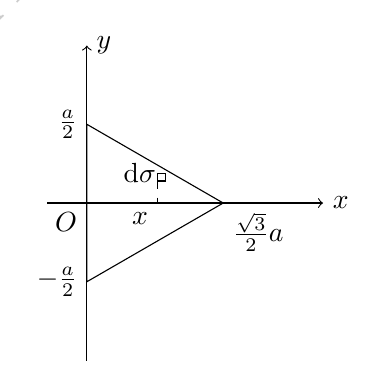
\begin{tikzpicture}
	\zbj{-0.5}{3}{-2}{2}
	\draw (0,-1) node[left] {$ -\frac{a}{2} $}
	-- (0,1) node[left] {$ \frac{a}{2} $}
	-- (1.732,0) node[below right] {$ \frac{\sqrt{3}}{2}a $}
	-- cycle;
	\draw [dashed](0.9,0.28) -- (0.9,0);
	\node[dashed,below left] at (0.9,0) {$ x $};
	\draw (0.9,0.280) rectangle (1,0.38) node [left]{$\di{\sigma}$};
	\end{tikzpicture}
	\caption{练习5示意图}\label{fig:c4-t5}
\end{figure}

按转动惯量之定义作积分,可得:
\begin{align*}
J&=2J_1=2\iint\limits_{\sigma_1}x^2\cdot\di{m}=2\iint\limits_{\sigma_1}x^2\cdot\left(m\frac{\di{\sigma}}{\frac{\sqrt{3}}{4}a^2}\right)\\
&=\frac{8m}{\sqrt{3}a^2}\int_0^{\frac{\sqrt{3}}{2}a}\di{x}\int_0^{\frac{1}{2}a-\frac{\sqrt{3}}{3}x}x^2\di{y}=\frac{8m}{\sqrt{3}a^2}\int_0^{\frac{\sqrt{3}}{2}a}\di{x}\left(\frac{1}{2}ax^2-\frac{\sqrt{3}}{3}x^3\right)\\
&=\frac{8m}{\sqrt{3}a^2}\left.\left(\frac{1}{6}ax^3-\frac{\sqrt{3}}{12}x^4\right)\right|_0^{\frac{\sqrt{3}}{2}a}=\frac{8m}{\sqrt{3}a^2}\left(\frac{\sqrt{3}}{16}a^4-\frac{3\sqrt{3}}{64}a^4\right)\\
&=\frac{8m}{\sqrt{3}a^2}\frac{\sqrt{3}}{64}a^4=\frac{1}{8}ma^2
\end{align*}

即$ J=\frac{1}{8}ma^2 $.

\exercise{6}A

\solve 直观上理解,$ \sigma(\theta) $在$ \theta=\frac{\pi}{2} $时最大,在$ \theta=0 $或$ \theta=\pi $时最小,此即球面质量更多地分布在赤道附近,两极附近质量面密度小。由于赤道附近距离$ z $轴距离更大,因此分布不均匀的球面转动惯量更大,A正确。\par
通过计算也可以得到相同的结论,此处不再赘述。

\exercise{7}A

\solve 碰撞过程中$ \Delta t\to 0 $,小球和系杆组成的系统受到4个力:重力,支持力(与重力相互抵消),O点对杆的支持力,O点对杆的摩擦力。因此系统角动量守恒(详细分析可见选择题3的“注”部分),有:
\[0+rmv=\left[\frac{1}{12}ml^2+m\left(\frac{l}{2}\right)\right]^2\omega\]
解得$\omega=\dfrac{3v}{2l}$.

\exercise{8}C

\begin{figure}[htbp]
	\centering
	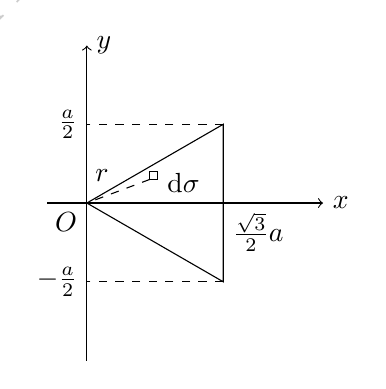
\begin{tikzpicture}
	\zbj{-0.5}{3}{-2}{2}
	\draw (0,0)-- (1.732,1) -- (1.732,-1) -- cycle;
	\draw[dashed] (1.732,1) -- (0,1) node[left] {$ \frac{a}{2} $};
	\draw[dashed] (1.732,-1) -- (0,-1) node[left] {$ -\frac{a}{2} $};
	\node[below right] at (1.732,0) {$\frac{\sqrt{3}}{2}a$};
	\draw (0.8,0.3) rectangle (0.9,0.4);
	\draw [dashed](0.8,0.3) -- node[above left] {$ r $} (0,0);
	\node [below right] at (0.9,0.5) {$\di{\sigma}$};
	\end{tikzpicture}
	\caption{练习8参考图}\label{fig:c4-t8}
\end{figure}

\solve 参考图\ref{fig:c4-t8},微元$ \di{\sigma} $到轴(就是到原点)的距离为$ \sqrt{x^2+y^2} $。由于积分域关于$ x $轴对称,被积函数关于$ y $为偶函数,因此$ J=2J_1 $,$ J_1 $为第一象限部分的转动惯量。则
\begin{align*}
J&=2J_1=2\iint\limits_{\sigma_1}\left(m\frac{\di{\sigma}}{\frac{\sqrt{3}}{4}a^2}\right)(x^2+y^2)\\
&=\frac{8m}{\sqrt{3}a^2}\int_0^{\frac{\sqrt{3}}{2}a}\di{x}\int_0^{\frac{\sqrt{3}}{3}x}(x^2+y^2)\di{y}
\end{align*}
进一步计算\footnote{可参考本章练习5中类似积分式的计算过程。}可得$ J=\frac{5}{12}ma^2 $.

\exercise{9}A

\solve 由动量矩定理易知A正确。BCD均为充分条件。小球在绳子的束缚下绕定点做匀速圆周运动,则所受合外力不为0(绳子的拉力),B错误,且小球受到的重力和支持力对定点的力矩均不为0,因此受到了外力矩的作用,C错误。对于D,可令$ J=t,\omega=\frac{1}{t} $,则$ L=J\omega=1 $,角动量守恒,但转动惯量和角速度都在随时间变化,因此D错误。

\exercise{10}A

\solve 卫星做匀速圆周运动,则$ m,v,r $均不变,$ \vec{r}\times\vec{v} $的方向也不变,因此角动量守恒。卫星与地球的万有引力与卫星的运动方向恒垂直,因此卫星与地球构成的系统的内力(万有引力)不做功,同时又不受外力作用,因此卫星的动能守恒。

\section{填空题}
\exercise{11}$\frac{3M}{ma} \hspace{2em} \frac{18M^2}{m^2a^3}t^2$

\solve 本题中转动方向固定,用标量形式计算即可。首先有
\[\beta=\frac{M}{J}=\frac{6M}{ma^2}\]
开始时$\omega=0$,故对$\beta$积分即可依次得到
\begin{gather*}
\omega=\frac{6M}{ma^2}t\\
v=\omega r=\frac{6M}{ma^2}t\times\frac{a}{2}=\frac{3M}{ma}t
\alpha_{\tau}=\dy{v}{t}=\frac{3M}{ma}\\
\alpha_n=\frac{v^2}{r}=\frac{\left(\frac{3M}{ma}t\right)^2}{\frac{a}{2}}=\frac{18M^2}{m^2a^3}t^2
\end{gather*}


\exercise{12}$\frac{1}{12}mR^2\omega_0^2$

\solve 圆柱所受合外力为摩擦力$f$,效果使得圆柱的质心运动速度$ v_c $增大。

圆柱所受合外力矩为摩擦力矩$ M_f $,效果使得圆柱的角速度$ \omega $减小。

圆柱做纯滚动的瞬间,即$ v_c=\omega R $。因此求得$ v_c $和$ \omega $对时间的函数,解出$ t $即可。

对圆柱使用牛顿第二定律$F=ma$和转动定律$M=J\beta$,可得
\[\begin{cases}
a_c=\dfrac{f}{m}=\mu g&\Rightarrow v_c=0+\mu gt=\mu gt\\[0.5cm]
\beta=\dfrac{M}{J}=\dfrac{-\mu mgR}{\dfrac{1}{2}mR^2}=-\dfrac{2\mu g}{R}&\Rightarrow\omega=\omega_0+\beta t=\omega_0-\dfrac{2\mu g}{R}t
\end{cases}\]
代入纯滚关系式,有
\[\mu gt=\omega_0R-2\mu gt\]
解得$t=\frac{\omega_0R}{3\mu g}$,此时
$v_c=\mu g\frac{\omega_0R}{3\mu g}=\frac{\omega_0R}{3}$,$\omega=\omega_0-\frac{2\mu g}{R}\frac{\omega_0R}{3\mu g}=\frac{\omega_0}{3}$。由柯尼希定理,可算得
\[E_{\text{总}}=\frac{1}{2}mv_c^2+\frac{1}{2}J\omega^2=\frac{1}{2}m\left(\frac{\omega_0R}{3}\right)^2+\frac{1}{2}\left(\frac{1}{2}mR^2\right)\left(\frac{\omega_0}{3}\right)^2=\frac{1}{12}mR^2\omega_0^2\]

\exercise{14}$\frac{1}{8}Mg$

\solve 物体加速度$ a $与滑轮角加速度$ \beta $的关系为:
\[\beta=\frac{a}{R}=\frac{g}{4R}\]
对滑轮应用转动定律$M=J\beta$:
\begin{gather*}
TR=\frac{1}{2}MR^2\beta\\
\therefore T=\frac{MR^2}{2R}\frac{g}{4R}=\frac{1}{8}Mg
\end{gather*}

\exercise{15}$\frac{1}{2l}\left(\sqrt{\frac{3gl}{2}}+\frac{v_0}{2}\right)$

\solve 首先计算碰撞前杆的角速度,由机械能守恒:
\begin{gather*}
0+0=Mg(-\frac{l}{2}\sin 30^\circ)+\frac{1}{2}J\omega^2\\
\omega_1=\sqrt{\frac{Mgl}{4}\frac{2}{\frac{1}{3}Ml^2}}=\sqrt{\frac{3g}{2l}}
\end{gather*}

以杆和子弹为系统,在碰撞过程中,所受外力里只有O点对杆的支持力为无穷大(抵消子弹沿杆方向的速度),但该力产生的力矩为0,因此碰撞过程中系统角动量守恒,有:
\begin{gather*}
l\sin 30^\circ mv_0+J\omega_1=(J+ml^2)\omega\\
\therefore \omega=\frac{1}{2l}\left(\sqrt{\frac{3gl}{2}}+\frac{v_0}{2}\right)
\end{gather*}

\exercise{16}$\frac{1}{4}mR^2$

\solve 均匀圆形薄板对圆心的转动惯量$ J=\frac{1}{2}mR^2 $,由垂直轴定理,$ J=J_1+J_2 $,$ J_1,J_2 $分别为薄板对其自身一条直径的转动惯量(两条相互垂直的直径)。由于圆板为圆对称,对任意一条直径的转动惯量相同,因此$ J_1=J_2 $,则$ J_1=\frac{1}{2}J=\frac{1}{4}mR^2 $

\exercise{17}$J_1=J_2$

\solve 记薄板对垂直于自身并穿过中心的轴的转动惯量为$ J $。

由对称性,薄板分别相对于两条对角线的转动惯量相等,均为$J_1$;分别相对过其中心且平行于一边的轴的转动惯量也相等,均为$J_2$,如图\ref{fig:c4-t17}所示。

\begin{figure}[htbp]
	\centering
	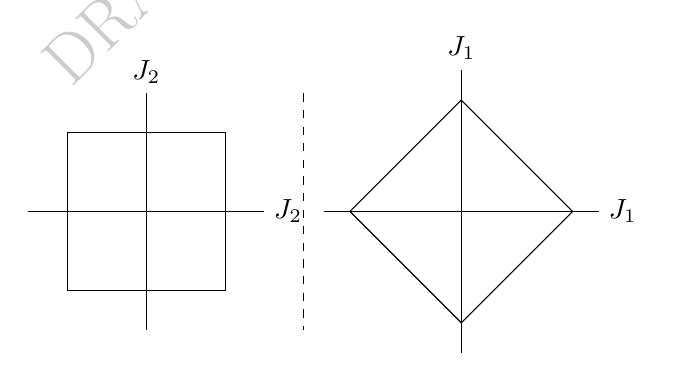
\begin{tikzpicture}
	\draw [rotate around={45:(4,0)}] (3,-1) rectangle (5,1);
	\draw (5.75,0) node[right] {$ J_1 $} -- (2.25,0);
	\draw (4,1.8) node[above] {$ J_1 $} -- (4,-1.8);
	\draw [dashed] (2,1.5) -- (2,-1.5);
	\draw (-1,-1) rectangle (1,1);
	\draw (1.5,0) node[right] {$ J_2 $} -- (-1.5,0);
	\draw (0,1.5) node[above] {$ J_2 $} -- (0,-1.5);
	\end{tikzpicture}
	\caption{练习17参考图}\label{fig:c4-t17}
\end{figure}

由垂直轴定理,$ J=2J_1=2J_2 $,因此$ J_1=J_2 $。

\exercise{18}75 rad/s

\solve 物块受到重力,支持力(相互抵消),绳的拉力。由于绳的向径与拉力的方向在同一条直线上,因此小物块所受合外力矩为0,角动量守恒。则:
\[(mR_1^2)\omega_0=(mR_2^2)\omega\]
解得$\omega=\frac{R_1^2}{R_2^2}\omega_0=\frac{0.5^2}{0.1^2}\times 3=75\ (\mathrm{rad/s})$。

\exercise{19}0

\solve 棒球沿直线飞行,则速度$ \vec{v} $的方向沿该直线,向径$ \vec{r} $的方向也沿该直线,因此角动量$ L=\vec{r}\times m\vec{v}=0 $。

\exercise{20}$2\sqrt{\frac{g\sin\theta}{3l}}$

\solve 由机械能守恒,可列出
\begin{gather*}
\hspace{1pt}2mg\left(\frac{l}{2}\sin\theta\right)+mg\left(-\frac{l}{2}\sin\theta\right)+0+0\\
=0+0+\frac{1}{2}\left(2m\left(\frac{l}{2}\right)^2\right)\omega^2+\frac{1}{2}\left(m\left(\frac{l}{2}\right)^2\right)\omega^2
\end{gather*}
解得$\omega=2\sqrt{\frac{g\sin\theta}{3l}}$。

\section{计算题}

\exercise{21}$\frac{m}{m+\frac{1}{2}M}\frac{Sg}{rl}$

\solve 对左端下垂链条应用牛顿第二定律$F=ma$,对上端链条和飞轮应用转动定律$M=J\beta$,右端下垂链条应用牛顿第二定律$F=ma$:
\begin{gather}
m\frac{l-\pi r+S}{2l}g-T_1=m\frac{l-\pi r+S}{2l}a\label{eq:c4-t21-1}\\
(T_1-T_2)r=\left(\frac{1}{2}Mr^2+m\frac{\pi r}{l}r^2\right)\beta\label{eq:c4-t21-2}\\
T_2-m\frac{l-\pi r-S}{2l}g=m\frac{l-\pi r-S}{2l}a\label{eq:c4-t21-3}
\end{gather}
代入$a=\beta r,(\ref{eq:c4-t21-1})+(\ref{eq:c4-t21-2})/r+(\ref{eq:c4-t21-3})$得:

\begin{align*}
m\frac{S}{l}g&=m\frac{l-\pi r}{l}\beta r+\left(\frac{1}{2}M+\frac{m\pi r}{l}\right)\beta r\\
&\left(m+\frac{1}{2}M\right)\beta r
\end{align*}
故$\beta=\frac{m}{m+\frac{1}{2}M}\frac{Sg}{rl}$.

\exercise{22}$a=\frac{2}{7}g$

\solve 人相对绳子加速度为0,绳子相对地面加速度为0,故人相对地面加速度为$a$。对人应用牛顿第二定律$F=ma$,对滑轮应用转动定律$M=J\beta$,对重物应用牛顿第二定律$F=ma$,可分别得到:
\begin{gather}
mg-T_1=ma\label{eq:c4-t22-1}\\
(T_1-T_2)R=\frac{1}{4}mR^2\alpha\label{eq:c4-t22-2}\\
T_2-\frac{1}{2}mg=\frac{1}{2}ma\label{eq:c4-t22-3}
\end{gather}
按$(\ref{eq:c4-t22-1})+\frac{(\ref{eq:c4-t22-2})}{R}+(\ref{eq:c4-t22-3})$合并三个等式,得
\begin{align*}
\frac{1}{2}mg&=\frac{3}{2}ma+\frac{1}{4}ma=\frac{7}{4}ma
\end{align*}
解得$a=\frac{2}{7}g.$

\exercise{23}$\Delta x=31.36m,\Delta\theta=78.4rad$

\solve 本解析取$ g=9.8m/s^2 $
\footnote{若取$g=10$m$/$s${}^2$,则相应的结果为$\Delta x=32m,\Delta\theta=80rad.$}
。以物体初始位置为原点,竖直向下为$x$轴建立坐标系。由能量守恒可得:
\[0+0+0=mg(-x)+\frac{1}{2}mv^2+\frac{1}{2}\left(\frac{1}{2}MR^2\right)\omega^2\]
即
\[gx=\frac{1}{2}v^2+\frac{1}{4}\frac{M}{m}v^2=\left(\dfrac12+\frac{M}{4m}\right)\cdot\left(\dy{x}{t}\right)^2\]
稍加变形得到
\[\sqrt\frac{g}{\frac{1}{2}+\frac{M}{4m}}\di{t}=\frac{\di{x}}{\sqrt{x}}\]
两边积分便得$\sqrt\frac{g}{\frac{1}{2}+\frac{M}{4m}}t=2\sqrt{x}+C$.代入$ t=0,x=0$可得$c=0$,故最终有
\[x=\frac{gt^2}{2+\frac{M}{m}}\]
代入$t=4$s,便得到
\begin{gather*}
\Delta x=x\left.\right|_{t=4}=\frac{16g}{2+\frac{15}{5}}=\frac{16}{5}g=31.36(\mathrm{m})\\
\Delta\theta=\left.\theta\right|_{t=4}=\frac{x}{R}=\frac{16g}{5\times 0.4}=8g=78.4(\mathrm{rad})
\end{gather*}

\note 这三道题是同一类型的问题,都可以用角动量定理和受力分析(如练习21、22)两种方法来求解。前者指的是,把系统中平动的链条、重物都看作都是转动的,写出其对滑轮转轴的角动量的表达式,用角动量定理解出角加速度,再求解其他物理量;后者则分别研究每一部分的转动或平动,分别列运动学基本方程,用角加速度和加速度的关系联系起来。但求解时可以发现,消去拉力后得到的就是角动量定理的表达式,而用第一种方法求拉力时,又要列出第二种方法的受力分析。所以说,两种方法本质是也一样的,如果只问与加速度有关的量就选用第一种。我们希望,读者在复习时,能使用角动量定理自己把以上三道题再做一遍,以体会其中深意,尤其是受力方向和角动量方向之区别,及所导致列式上的不同。如果要问诸如下降的距离等,也可采用练习23的解法,就可避过求加速度,也是一种好的思路。这是最基本的题型之一,问法相对固定,难度不大,老师希望通过这三道题来让同学们掌握这类题型。在2019年期末试题中,就有一道解答题是这个题型。

\exercise{24}$\frac{3m_2^2(v_1+v_2)^2}{m_1^2l\mu g}$

\solve 本题所述力矩,全部指对O点的力矩。

撞击前后瞬间,子弹和细棒组成的系统仅受O点支持力,因此合外力矩为0。由角动量守恒:
\[lm_2v_1+0=-lm_2v_2+\frac{1}{3}m_1l^2\omega\]
解得$\omega=\frac{3m_2(v_1+v_2)}{m_1l}$而摩擦力对O点力矩可计算为:
\[M=\int_{r=0}^{r=l}f\di{r}=\int_{r=0}^{r=l}\mu \di{m}g\di{r}=\int_0^l\mu gr\left(m_1\frac{\di{r}}{l}\right)=\frac{\mu m_1gl}{2}\]
又由于
\[M=J\dy{\omega}{t}=J\dy{\omega}{\theta}\dy{\theta}{t}=J\dy{\omega}{\theta}\omega\]
故有$\frac{M}{J}\di{\theta}=\omega\di{\omega}$。由$\theta=0$时$\omega=0$,对等式两边从$\theta=0$开始积分可得
\[\frac{M}{J}\theta=\frac{1}{2}\omega^2\]
故最终得到
\[\theta=\frac{\omega^2}{2}\frac{J}{M}=\frac{1}{2}\frac{9m_2^2(v_1+v_2)^2}{m_1^2l^2}\frac{\frac{1}{3}m_1l^2}{\frac{\mu m_1gl}{2}}=\frac{3m_2^2(v_1+v_2)^2}{\mu m_1^2gl}\]

\end{document}